\documentclass[12pt,a4paper]{report}
\usepackage[latin1]{inputenc}
\usepackage{amsmath}
\usepackage{amsfonts}
\usepackage{amssymb}
\usepackage[latin1]{inputenc}
\usepackage{amsmath}
\usepackage{amsfonts}
\usepackage{amssymb}
\usepackage{graphicx}
\usepackage{siunitx}
\usepackage{enumitem, nth}
\usepackage{mhchem}

\DeclareSIUnit\torr{torr}

\begin{document}

%%%%%%%%%%%%%%%%%%%%%%%%%%%%%%%%%%%%%%%%%%%%%%%%%%%%%%%%%%
%%%%%%%%%%%%%%%%%%%%%%%%%%%%%%%%%%%%%%%%%%%%%%%%%%%%%%%%%%
\thispagestyle{empty}

\begin{figure}[tl]

\includegraphics[scale=0.4]{fig/usydlogo.jpg}
\end{figure}

\begin{tabular}{c}
\\
\\
\\
\begin{huge}
\textbf{Nanofab work procedure}
\end{huge}
\\
\\
\rule{14cm}{1mm}
\end{tabular}

\vspace{2cm}

\begin{flushright}

\begin{Large}
\textbf{School of physics, Quantum group}\\
\vspace{0.5cm}
Last update: \today
\end{Large}
\end{flushright}

\vspace{4cm}

\noindent \textbf{Abstract}:\\
\textit{Description of each steps to manufacture quantum dots from a GaAs/AlGaAs chip.}\\

\begin{flushright}
Sylvain Blanvillain
\end{flushright}

\newpage
%%%%%%%%%%%%%%%%%%%%%%%%%%%%%%%%%%%%%%%%%%%%%%%%%%%%%%%%%%
%%%%%%%%%%%%%%%%%%%%%%%%%%%%%%%%%%%%%%%%%%%%%%%%%%%%%%%%%%

\chapter{Nanofabrication}

\section{Introduction}

\subsection{General steps to manufacture quantum dots}

The steps for manufacture are described below:\\

\begin{enumerate}[noitemsep]
\item Cleaving
\item Cleaning
\item Resist spinning
\item Photolithography (mesa pattern)
\item Resist developing
\item Mesa etching
\item Resist removal (5\,min sonication in NMP, rince with IPA)
\item Resist spinning (including cleaning on chuck)
\item Photolithography (ohmics pattern)
\item Resist developing
\item Plasma ash
\item Metal deposition (ohmics)
\item Lift-off
\item Annealing
\item Resist spinning
\item Electron Beam Lithography (fine gates)
\item Plasma ash
\item Metal deposition (fine gates)
\item Lift-off
\item Cleaning
\item Resist spinning
\item Photolithography (large gates)
\item Resist developing
\item Plasma ash
\item Metal deposition
\item Lift-off
\item Imaging
\end{enumerate}

\newpage

\subsection{Alignments DD V1}

\begin{figure} [h] \centering
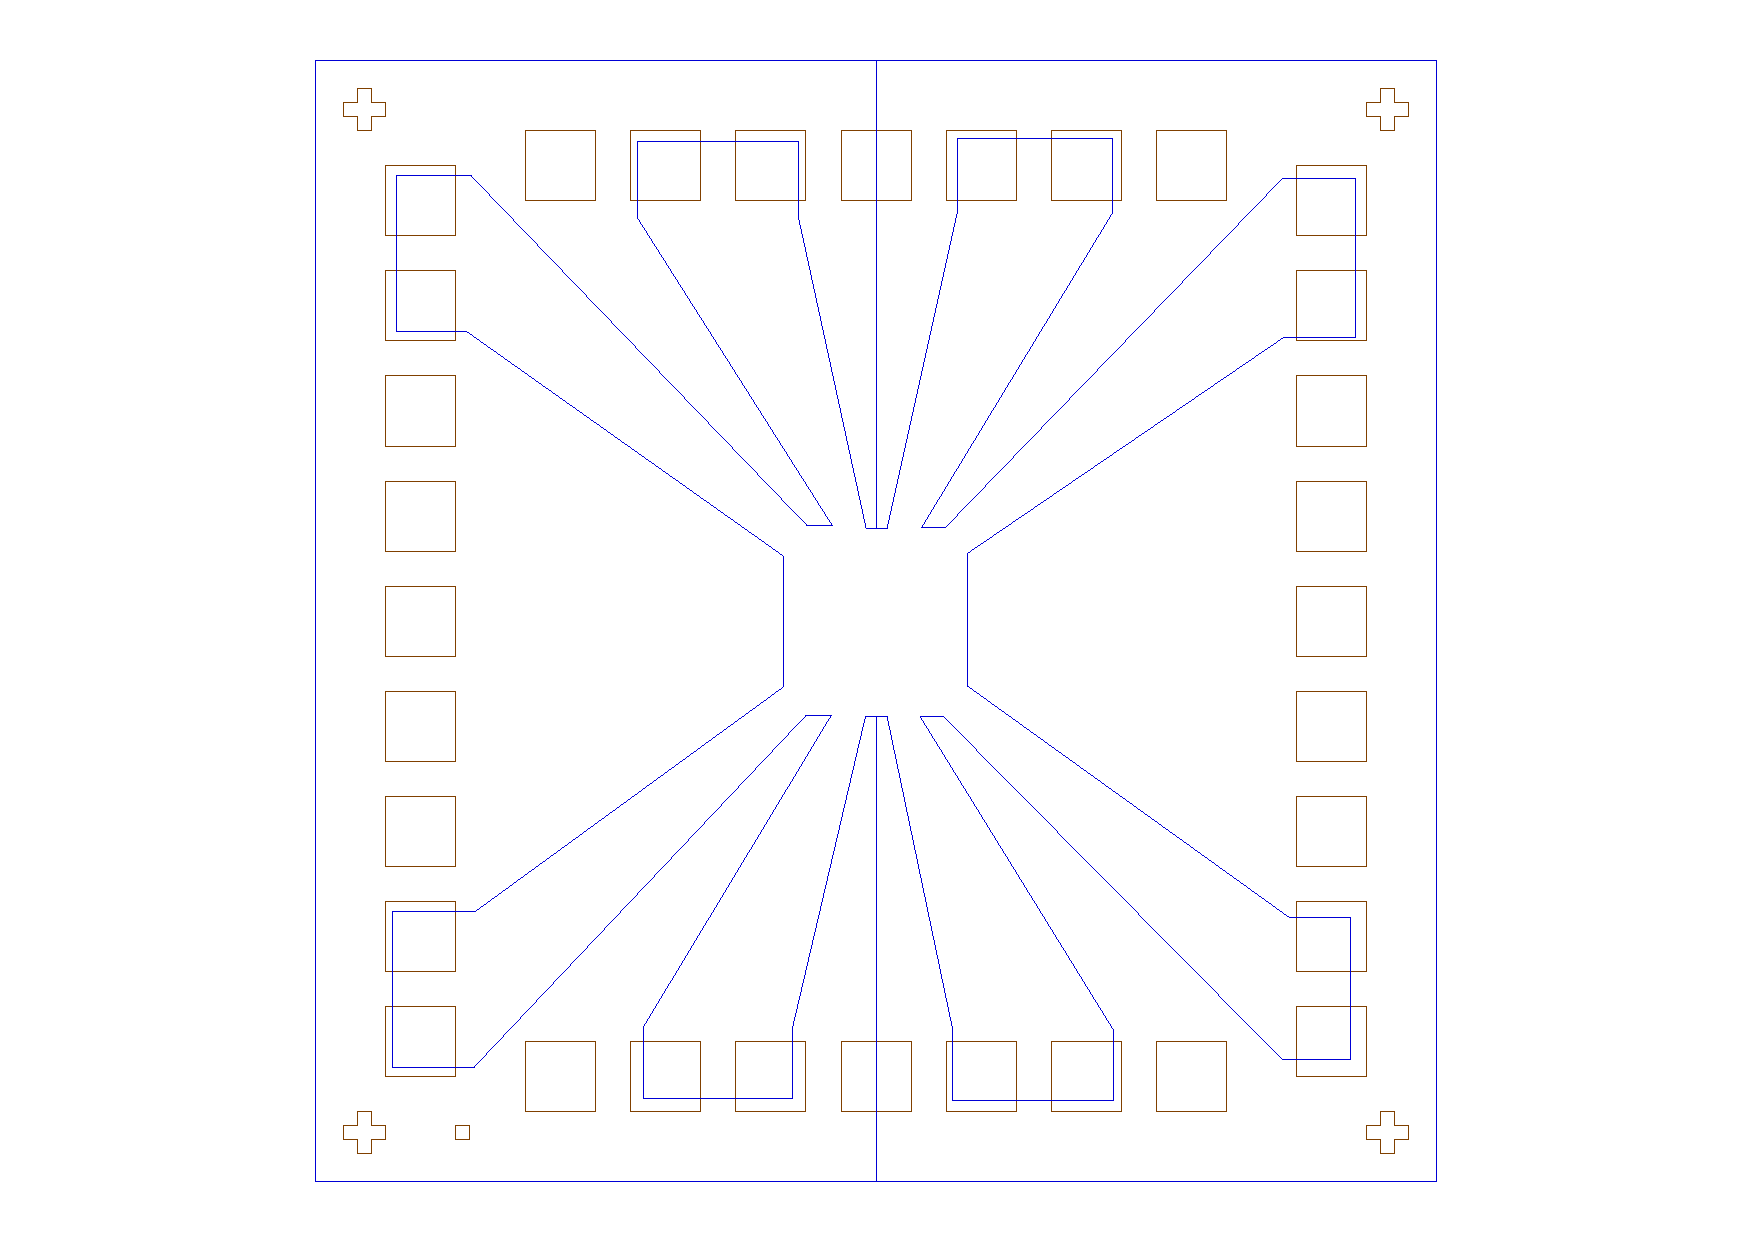
\includegraphics[scale=0.3]{fig/align1.pdf}
\caption{Alignment of the ohmics patern with the mesa patern.} \label{align1}
\end{figure}

\begin{figure} [h] \centering
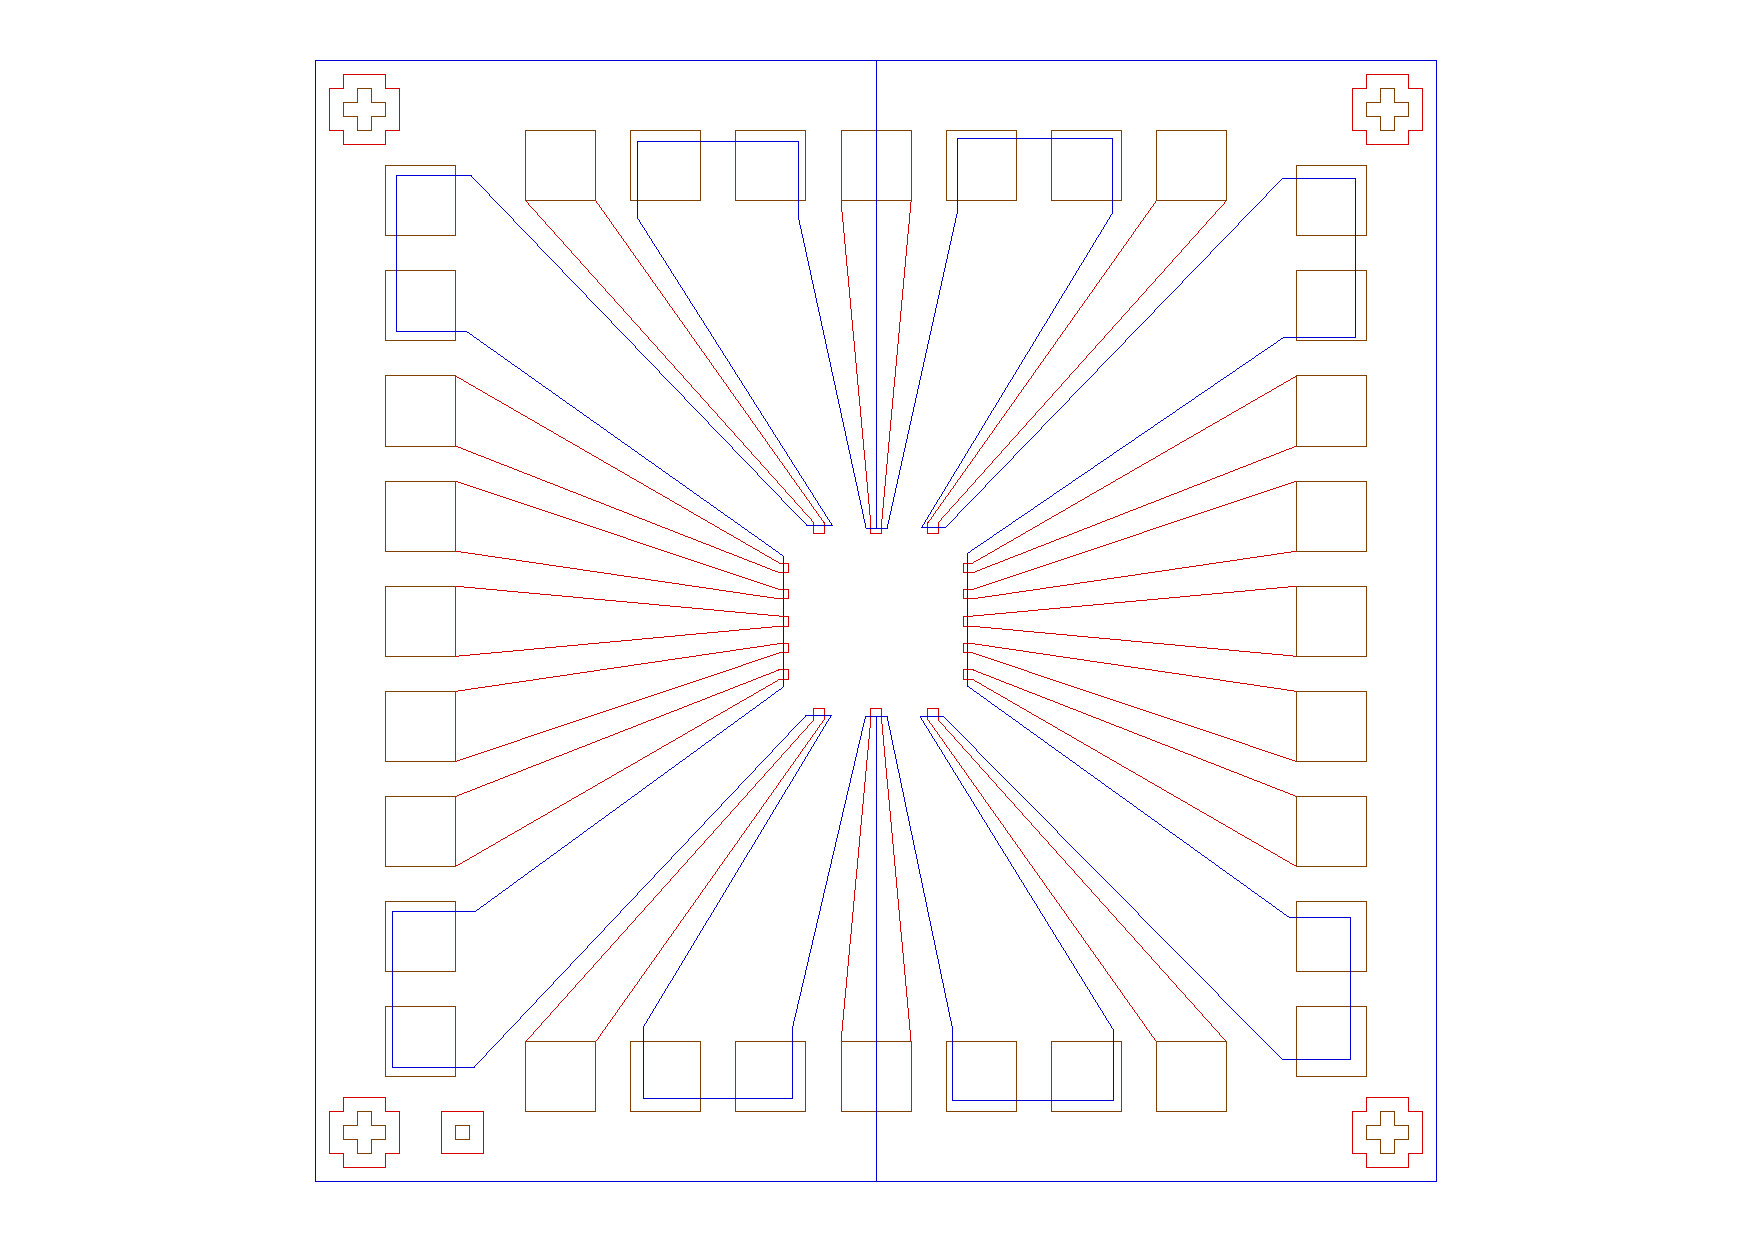
\includegraphics[scale=0.3]{fig/align2.pdf}
\caption{Alignment of the contacts with the ohmics and mesa paterns.} \label{align2}
\end{figure}

\newpage

\subsection{Alignments DD V2}

\begin{figure} [h] \centering
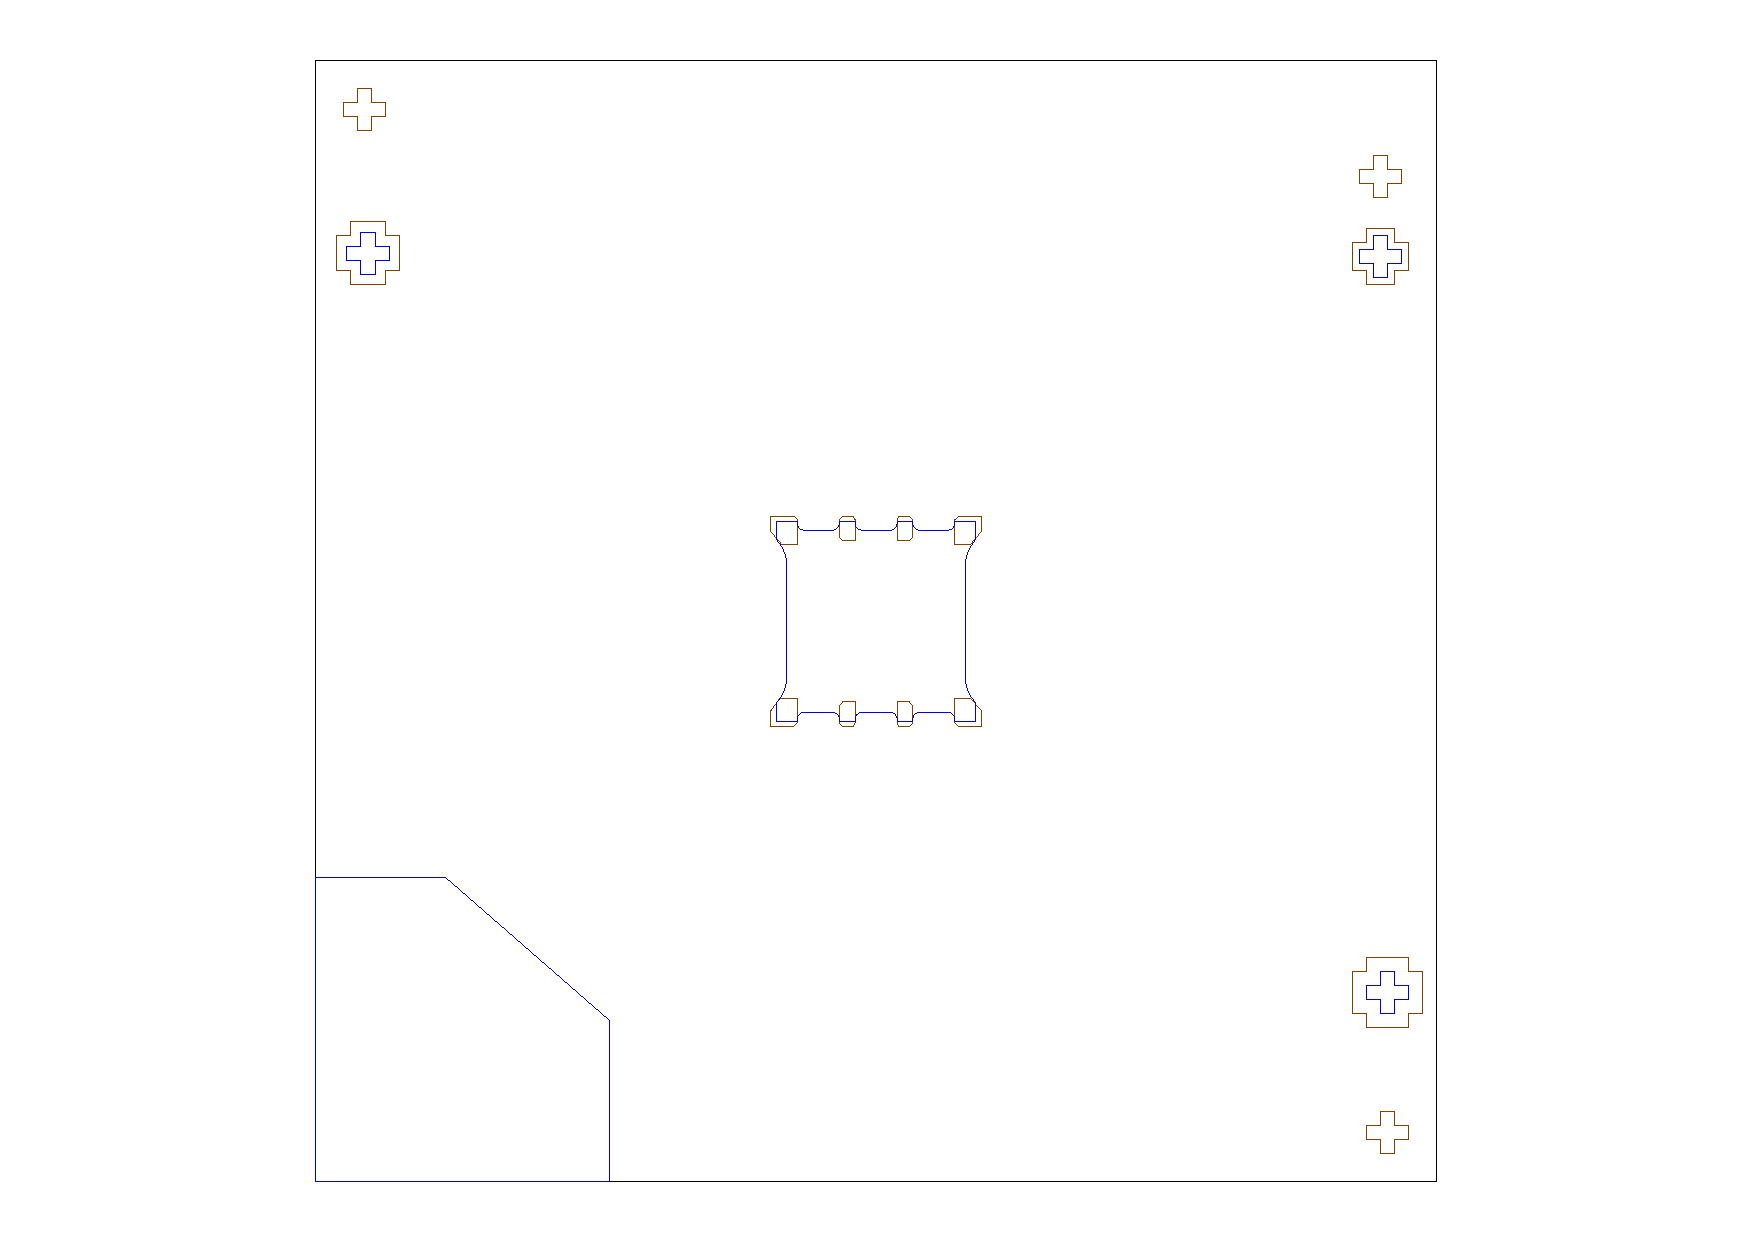
\includegraphics[scale=0.3]{fig/align1_1.pdf}
\caption{Alignment of the ohmics patern with the mesa patern.} \label{align1}
\end{figure}

\begin{figure} [h] \centering
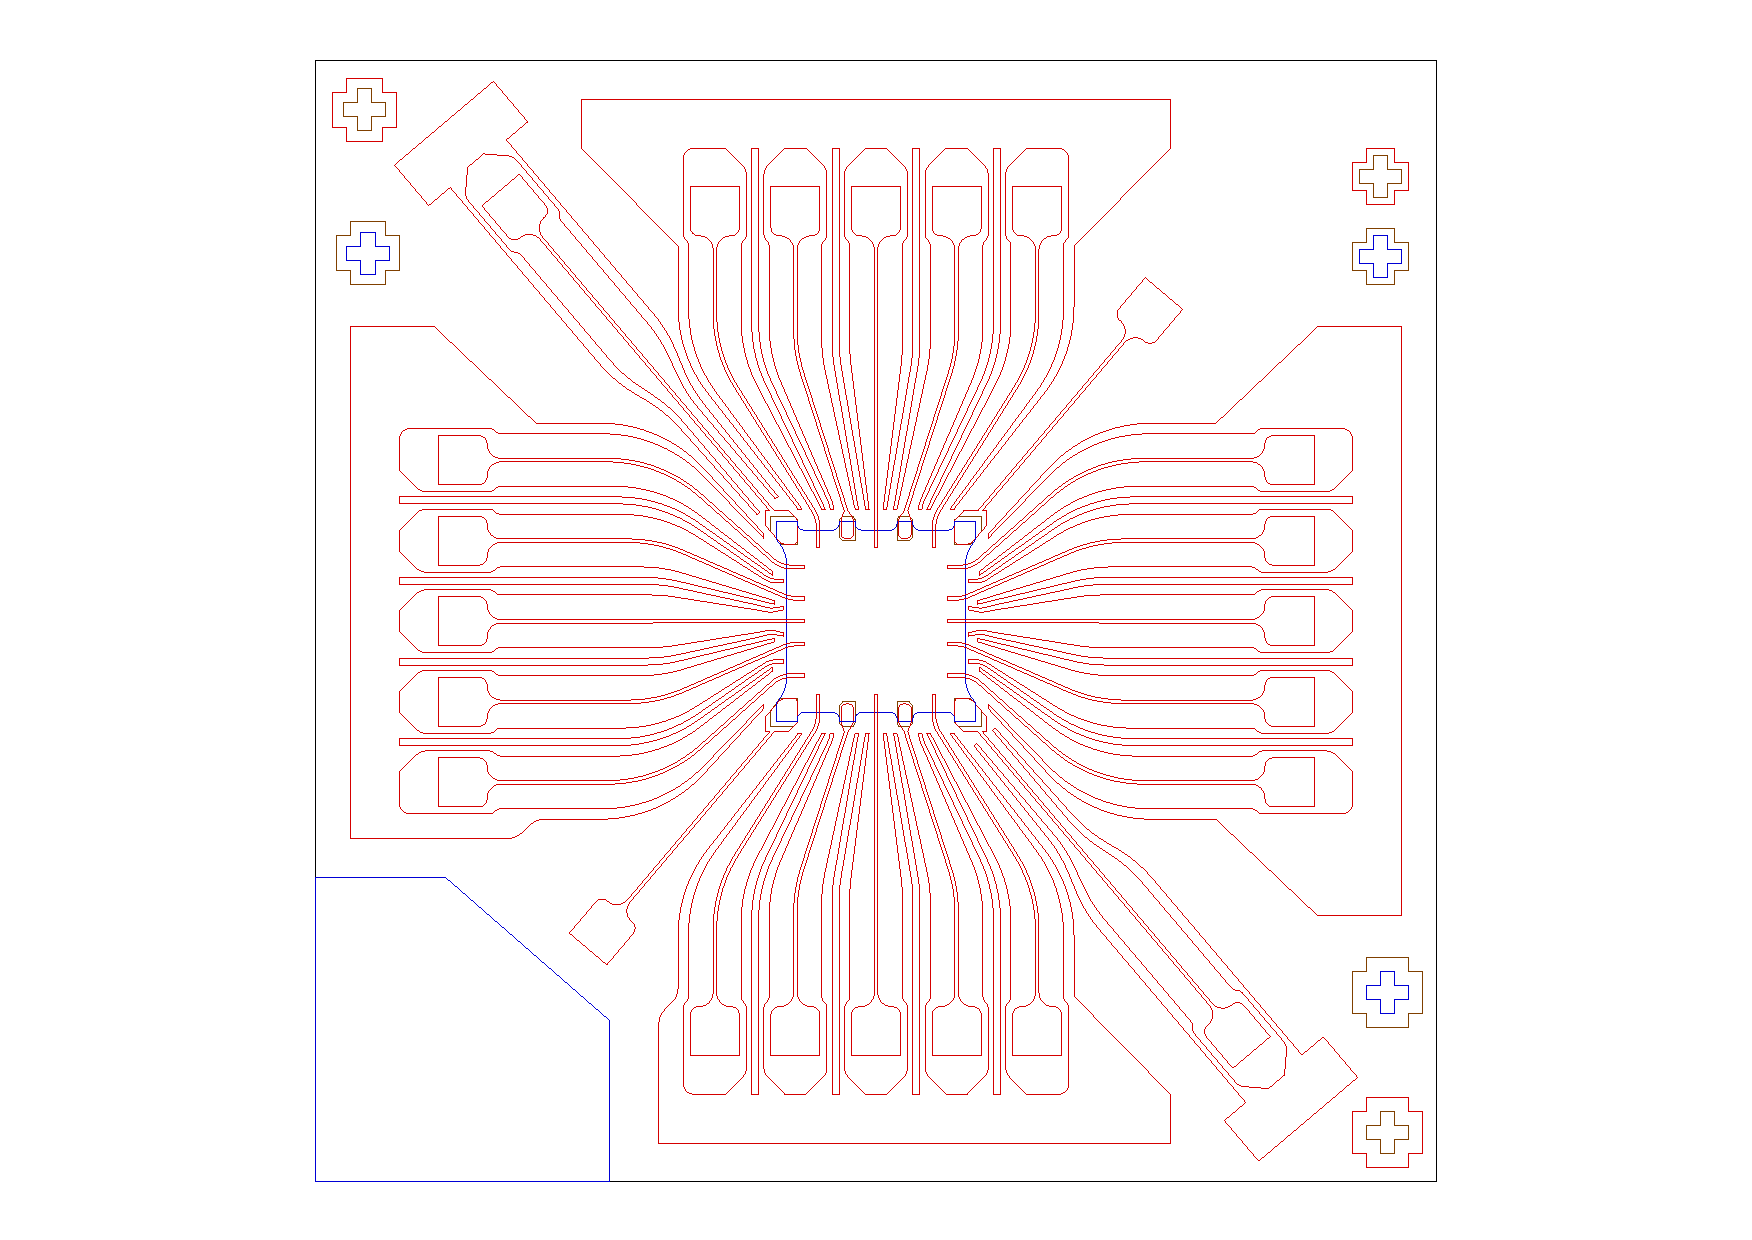
\includegraphics[scale=0.3]{fig/align2_1.pdf}
\caption{Alignment of the contacts with the ohmics and mesa paterns.} \label{align2}
\end{figure}



\newpage

\subsection{Dressing}
\begin{itemize}
\item mask
\item hair nest
\item suit
\item shoes (!on other side of bench!)
\item gloves
\item glasses
\end{itemize}

The clean room begin just after the bench in front of the door. DON'T SIT ON THE BENCH.

\subsection{Misc}

\begin{itemize}
\item Tools in lunch box
\item Clean everything you need/use
\item Write up EVERYTHING, make protocols
\item To quickly remove the water in beakers, spray IPA and blow dry
\item If the chip is flipped: clean and re-spin
\item Inside fume hoods, always manipulate beakers and 
chip on wipes (to avoid loosing the chip in holes).
\item If a solvent container is empty, open it and let it out gaz inside
the cupboard on the left hand side.
\item If the solvent waste is full, take an empty solvent container,
pour the solvent waste in it and put it in the bottom left hand
side shelve, on the left of the cupboard. Put a provided sticker
on it.
\end{itemize}

\newpage

\section{Cleaving}
\subsubsection{Aim}
Cut a desired geometry from the heterostructure
\subsubsection{Needs}
\begin{itemize}[noitemsep]
\item Round shape paper filter (always manipulate on it).
\item 2 glass slides
\item diamond pen
\item heterostructure
\item clean gloves (double glove)
\end{itemize}
\subsubsection{Steps}
\begin{enumerate}
\item Write on the logbook which part of the heterostructure you are going to take (name, date, location, what for...).\\
Label your part on the logbook:\\
h(hetero)/j(junk).date(200411).initials(sb).part nb(01...)
\item Take 2 glass parts, put the heterostructure on it.
\item Scratch the chip with the diamond pen (length of scratch $<$ \SI{1}{\milli\meter}) at the wanted chip length.\\
The dimensions of the chips are:
$5 \times 2.5$ \si{\milli\meter}
\item If a wafer needs to be cut, do a scratch with the diamond pen on both ends of the slide.\\
(Note: We can use the upstairs custom cleaving device as well.)
\item Balance the GaAs chip on the glass with the scratch aligned with the edge of the glass.
\item Press GaAs with edge of finger to cleave it.
\item The cleave should be clean and along the scratch direction. Check under microscope.
\item Choose a corner as a reference according to scratches.
\item Label the position of the chip in the box, and record details in log book.
\item Put the filter paper in the contaminated bin.
\end{enumerate}

\newpage

\section{Cleaning}

\subsubsection{Aim}
Remove any dust from the chip

\subsubsection{Needs}
\begin{itemize} [noitemsep]
\item NMP
\item Isopropanol (IPA)
\item clean tweezers
\item wipes
\item beakers for IPA, NMP
\end{itemize}

\subsubsection{Steps}
\begin{enumerate}
\item Warm up a hot plate to \SI{200}{\celsius}
\item Fill beakers with NMP and IPA with enough liquid to make it stand in the sonicator.
\item Put GaAs face up in NMP. Warm for 10 min at \SI{70}{\celsius} (Hot plate should be at correct temperature already).
\item Add some water to the sonicator if needed.
\item Sonicate for 5 min (press button in middle of sonicator to turn on) in NMP.
\item Move chip to IPA and sonicate in IPA for 5 min.
\item Blow dry with nitrogen on wipe while holding the chip with tweezers.
\item Bake on center of hot plate for 5 min at \SI{200}{\celsius}.
\item Put chip back in box.
\item Pour solvents in waste solvent container, and rinse beakers with IPA and blow dry.
\end{enumerate}

\subsubsection{Misc}
\begin{itemize}
\item Put filter papers between box and beakers, in case the chip drops
\item !don't place acetone or IPA on the hot plates!
\item Clean tweezers
\end{itemize}

\newpage

\section{Resist spinning}

\subsubsection{Aim}
Dispense a homogeneous layer of resist on the chip

\subsubsection{Resist Stack}
The resist stacks for various steps of processing are as follows:
\begin{description}[noitemsep, nolistsep, leftmargin=\parindent, labelindent=\parindent]
\item[Mesa Etch] \hfill
  \begin{itemize} [noitemsep, nolistsep]
    \item AZ6612
  \end{itemize}
\item[Ohmics] \hfill
  \begin{itemize} [noitemsep, nolistsep]
    \item AZ6612
    \item LOR 5A
  \end{itemize}
\item[Fine Gates] \hfill
  \begin{itemize} [noitemsep, nolistsep]
    \item PMMA A3
  \end{itemize}
\item[Optical Gates] \hfill
  \begin{itemize} [noitemsep, nolistsep]
    \item AZ6612
    \item LOR 5A
  \end{itemize}
\end{description}

\subsubsection{Needs}
\begin{itemize} [noitemsep]
\item check everything is clean
\item IPA
\item pipette
\item resist AZ6612, LOR 5A, PMMA A3
\item timer
\end{itemize}

\subsubsection{Programming}
\begin{enumerate}
  \item Hit \boxed{recipe}, then recipe number (\boxed{1}).
  \item If the recipe needs to be cleared (too many steps) hit \boxed{recipe}, \boxed{clear} and then the recipe number (\boxed{1}).
  \item Hit \boxed{step}, then the step number (\boxed{1}).
  \item Hit \boxed{speed}, then set up the rotation speed (500rpm for step 1). Hit \boxed{enter} when done.
  \item Hit \boxed{speed}, then set up the ramp slope (500rpm/sec ramp for step 1). Hit \boxed{enter} when done.
  \item Hit \boxed{terminate}, then set up the duration of the step (5.0 sec for step 1). Hit \boxed{enter} when done.
  \item Hit \boxed{step}, choose the step number and repeat as many times as required.
  \item To finish, hit \boxed{step}, then \boxed{0}.
\end{enumerate}

\subsubsection{Recipes}
\begin{description}[nolistsep, noitemsep]
\item {LOR 5A}
  \begin{enumerate}
  \item 500rpm for 5 sec, 500 rpm/sec ramp.
  \item 10000rpm for 1 sec, 10000 rpm/sec ramp.
  \item 2500rpm for 60 sec, 7500 rpm/sec ramp.
  \item (finish) 0 rpm for 0 sec, 2000 rpm/sec ramp.
  \item Bake for 5 min at \SI{170}{\celsius}
  \end{enumerate}
\item {AZ6612}
  \begin{enumerate}
  \item 500 rpm for 5 sec, 500 rpm/sec ramp.
  \item 10000 rpm for 20 sec, 4000 rpm/sec ramp.
  \item 4000 rpm for 20 sec, 4000 rpm/sec ramp.
  \item (finish) 0 rpm for 0 sec, 2000 rpm/sec ramp.
  \item Bake for 60 sec at \SI{95}{\celsius}
  \end{enumerate}
\item {PMMA A3}
  \begin{enumerate}
  \item 500 rpm for 5 sec, 500 rpm/sec ramp.
  \item 9000 rpm for 5 sec, 4000 rpm/sec ramp.
  \item 6000 rpm for 30 sec, 4000 rpm/sec ramp.
  \item (finish) 0 rpm for 0 sec, 2000 rpm/sec ramp.
  \item Bake for 90 sec at \SI{180}{\celsius}
  \end{enumerate}
\end{description}

\subsubsection{Steps}
\begin{enumerate}
\item Put the chip at the center of the chuck (ensure there is no wobbles).
\item Check the recipe.
\item Make sure other chips/tools are protected from projections.
\item Take some droplets of resist with a pipette. Put the pipette with resist in its bag.
\item Spin clean the chip:
\begin{enumerate}
\item Spin at 4000rpm.
\item Spray 5 seconds of Acetone
\item Spray 5 seconds with Acetone and IPA (don't let Acetone dry)
\item Spray 5 seconds with IPA
\item Blow dry while spinning
\end{enumerate}
\item Place 2-3 drops of resist with the pipette on the chip during the 500 rpm spin
\item Always put the pipette back in its bag, wait for the spinning to stop
\item Bake the chip
\item Put the chip back in its box
\item Clean the spinner (!no liquid in vacuum hole!): use wipes with acetone to clean the chuck, protections, bench.
\end{enumerate}

\subsubsection{Misc}
\begin{itemize}
\item Don't put liquid in the spinner vacuum hole when cleaning.
\item Resist AZ6612, 12 means \SI{1.2}{\micro\meter}. (Measured depth closer to \SI{800}{\nano\meter})
\item If you will be spinning LOR 5A turn on the hot plate before you start. It takes about 10 minutes to warm up.
\item Note that the vacuum only turns on while the spinner is running. Don't spray before or after the spinner has stopped.
\end{itemize}

\newpage

\section{Photolithography}

\subsubsection{Aim}
Weaken the non-exposed resist

\noindent \textbf{Need}:
\begin{itemize}[noitemsep]
\item chip
\item tweezers
\item clean mask (upper side: silver, bottom side: chrome)
\end{itemize}

\subsubsection{Steps}
\begin{enumerate}
\item At the bottom left part, check that the device is in:
\begin{itemize}[nolistsep, noitemsep]
\item Constant power mode ($\neq$ constant intensity)
\item Watts mode ($\neq$ \si{\milli\watt\per\square\centi\meter})
\end{itemize}
\item Turn power on lamp on (bottom right switch)
\item Press and hold the start button (around 2 sec) until the sound `wiiiii' vanishes.
Device is powered up when levels on left/bottom gauges have moved from zero.
\item Wait 10 min for the lamp to warm up
\item Switch on the power to the aligner
\item At the bottom left, set up modes to:
\begin{itemize}[nolistsep, noitemsep]
  \item Constant Intensity
  \item \si{\milli\watt\per\square\centi\meter}
\end{itemize}
\item Check that the aligner is indicating pressure mode
\item Hit \boxed{exposure-test} switch to make place and check the exposure properties
\item Check the exposure time and intensity:
\begin{itemize}[nolistsep, noitemsep]
  \item Exposure time at 1.6 sec
  \item Check the wavelength is \SI{365}{\nano\meter}
  \item Hit \boxed{shutter} on/off to check the power which should be 10 mW (to be read on one of the bottom left gauges)
  \item Hit \boxed{pulse} to check and save the exposure time
  \item After the pulse, the lamp will move out of the way and the microscope into position
\end{itemize}
\item Hit the mask \boxed{load} button to move the microscope out of the way
\item Put the chip on the right stage
\item Hit \boxed{load} to load the chip at the place where the mask will be
\item Manually position the mask above the chip without touching the chip and without lying the mask on the vacuum line
\item Unload the chip (hitting \boxed{clear})
\item Put the mask on the vacuum line
\item Hit \boxed{vac} to clamp the mask with vacuum
\item Load the chip
\item Swing the microscope back (mask \boxed{load})
\item Wait for the light corresponding to "contact" to be green (chip can be moved) and not red (chip must not be moved).
(Note: if the light does not illuminate, swing the microscope out and back)
\item Turn the \boxed{lamp~saver} off
\item Adjust the chip position under the mask using joysticks (take care of the maximum displacement range of joysticks)
\item Press \boxed{contact} to make the mask in contact with the chip
\item Press \boxed{exposure}. The chip will automatically swing out
\item Unload the chip, put it back in its box
\item Press \boxed{load} to put the microscope on the right
\item Press \boxed{vac} to free the mask
\item Put the mask in its box, ensure it is firmly closed
\item Turn off powers on top, then bottom of the device
\item Switch modes to:
\begin{itemize}[nolistsep, noitemsep]
\item Constant Power
\item Watts
\end{itemize}
\end{enumerate}
\newpage
\subsubsection{Misc}
\begin{itemize}
\item Exposed resist is removed (negative resist)
\item If the 'separate' light does not illumiate, move the microscope back and forward (hit the mask \boxed{load} button twice).
\item To clean the mask, spray IPA on both sides, gently wipe with clean room wipes. Blow dry with nitrogen.
\item Turn the lamp on 5 mins before you need to align, it needs time to start up.
\end{itemize}
\newpage

\section{Resist developing}

\textbf{Aim}:
Remove the resist weakened by photolithography

\subsubsection{Needs}
\begin{itemize}[noitemsep]
\item exposed chip
\item resist developer MIF300
\item MIF300 beaker
\item water beaker
\end{itemize}

\subsubsection{Steps}
\begin{enumerate}
\item Pour developer in the appropriate beaker
\item Prepare a beaker of DI water
\item Put the chip in the developer for exactly 45 sec
\item While in developer move the chip around gently. always hold the chip in tweezers.
\item Put the chip in water for 30sec to rince it.
\item Blow dry 10 long seconds
\item Check under microscope
\item If islands of resist remains, repeat the operation for a shorter time
sharps etched edges mean success
\item \underline{Throw the developer in the drain} and rinse beakers with water and IPA
\end{enumerate}

\subsubsection{Misc}
\begin{itemize}
  \item The aim is to get sharp well defined edges, of the same size as on the mask.
  \item If features are smaller than on the mask, you can either increase exposure time or increase development time.
  \item If features are too large, either decrease exposure time or development time.
  \item The size of the undercut on LOR is defined by the amount of time it spends in developer (and bake temperature).
  It is not affected by exposure time.
\end{itemize}
\newpage

\section{Dektak}

\subsubsection{Aim}
Measure the thickness of remaining resist. Set up a reference to measure the etch of the mesa.

\subsubsection{Steps}
\begin{enumerate}
\item Draw the pattern of your mesa, or any geometry you want to measure the depth. Mark and number where measurement will be made.
\item Turn Dektak on 10 min before use
\item Clean the plate
\item Position the chip under the camera
\item Hit \boxed{program}, \boxed{enter} in 'scan menu'
\item Set up:
\begin{itemize}[nolistsep, noitemsep]
  \item Scan length (\SI{200}{\micro\meter})
  \item Scan speed (medium)
  \item Scan range (\SI{655}{\kilo\angstrom})
  \item Scan force (between 4 (noisy) and 9)
\end{itemize}
\item Hit \boxed{scan} to do your scan
\item Hit \boxed{ref} (\boxed{meas}) to manipulate the reference (measurement) marker.
\begin{itemize}[nolistsep, noitemsep]
  \item \noindent \boxed{lvl}: remove a slope in measurements between the ref and meas cursors
  \item \boxed{Avg HT}: average of measurements between markers
  \item \boxed{Max HT}: difference between the maximum and minimum between markers
  \item \boxed{\Delta ASH}: average step height
  \item \boxed{PT}: print
\end{itemize}
\item Always draw where you did your measurements, the thickness of the resist will normally vary by \SIrange{10}{100}{\nano\meter} across the chip
\end{enumerate}

\subsubsection{Misc}
\begin{itemize}
\item After developping the resist, the height of the remaining resist should be around \SI{12}{\kilo\angstrom}
\item If measurements are 'bumpy', try increasing the force
\item If measurements look `strange' or incoherent, first re-try a measurement
\end{itemize}
\newpage

\section{Mesa etching}

\textbf{Aim}:
Remove the 2DEG layer which is not under the mesa pattern. The thickness to remove is around \SI{210}{\nano\meter} for Sandia, and \SI{110}{\nano\meter} for Gossard
and \SI{130}{\nano\meter} for Manfra.

\subsubsection{Needs}
\begin{itemize}[noitemsep]
\item Mesa Etch, DI Water beakers
\item measuring cylinders for \ce{H2O2}, \ce{H2SO4}, \ce{H2O}
\item one big beaker
\item 2 pipettes
\item timer
\end{itemize}

\subsubsection{Steps}
\begin{enumerate}
\item Open the water tap and let it flow
\item Be sure your gloves are fitted properly (you might want to double glove)
\item Prepare the acid etch solution. Remember \underline{always acid in water}. The recipe is:
  \begin{itemize}
  \item 240ml of \ce{H2O}
  \item 8ml of \ce{H2O2}
  \item 1ml of \ce{H2SO4}
  \end{itemize}
\item Rinse used beakers and measuring cylinders thoroughly. Acids and \ce{H2O2} go down the drain, not in the solvents.
\item Mix acid solution with tweezers
\item Put some of the solution in the 'mesa etch beaker'
\item Put the chip in the solution for 50 sec (the etch rate should be around 2nm/sec)
\item Put the chip in water, rinse thoroughly for 30 sec.
\item Blow dry
\end{enumerate}
\subsection{Measure the etch depth}
\begin{itemize}
\item Use the Dektak to measure the depth of the etch
\item Measure at the same points than when the height of the resist was measured. The height of the resist is not uniform around the chip so it
is important to use the same locations when measuring.
\item Use measurements before etch to compute the etching rate (depth after etch (\AA) - depth before etch (\AA))/ etching time (sec) = etching rate ((\AA)/sec)
\item Deduce the etching time needed to etch at a total depth of 210 nm (etching more will reveal impurities)
\end{itemize}
\newpage

\section{Metal lift-off}

\textbf{Aim}:
Remove the remaining resist and metal after deposition

\subsubsection{Needs}
\begin{itemize}[noitemsep]
\item NMP and corresponding beaker
\item IPA and corresponding beaker
\item Acetone and corresponding beaker
\item water and corresponding beaker
\item sonicator
\end{itemize}

\subsubsection{Steps}
\begin{enumerate}
\item Warm NMP for at least 10 min to \SI{70}{\celsius}.
\item Ensure that there is sufficient water in the sonicator (should come well over stage).
\item Place chips in warm NMP for 1 hour.
\item Sonicate at minimum power for \SI{5}{\second}. (Can use medium power, \SI{10}{\second} for ohmics).
\item While in NMP, check to see if liftoff looks successful. Do not allow the chip to dry.
\item If unsuccessful either repeat above steps, or spray across surface of chip with acetone. Repeat
as many times as necessary.
\item Put chip in IPA beaker, spray with bottle.
\item Blow dry well.
\end{enumerate}

\noindent \textbf{Misc.}:
\begin{itemize}
\item If liftoff was unsuccessful, you can attempt the above steps again. However once dry, metal becomes
much more difficult to lift off.
\item Spraying vigorously with acetone can help liftoff along.
\item If gates are broken, check the edges under SEM. Bright white edges suggests the metal was ripped
off during liftoff and is an indicator of insufficient resist depth.
\end{itemize}
\newpage

\section{\ce{O2} Plasma Ashing}
\subsubsection{Aim}
Remove organic contaminants and resist remnants on the surface of the device

\subsubsection{Needs}
\begin{itemize}[noitemsep]
  \item Chip with developed resist
\end{itemize}

\subsubsection{Steps}
\begin{enumerate}
  \item Turn on the \boxed{\ce{N2}~Purge} switch to begin nitrogen flowing (even if already vented).
  \item Open chamber (door should open easily) and place chips onto the glass sample stage.
  \item Close the chamber door and turn on mechanical pump switch while firmly pushing against the door. Note that
  the \boxed{\ce{N2}~Purge} switch should still be on and should be left on. It will automatically turn off when the pump starts.
  \item Wait until the chamber pressure is $< \SI{85}{\milli\torr}$ (approx 15 mins). Note, $< \SI{70}{\milli\torr}$ is ideal.
  \item Flick the \boxed{GAS1~Oxygen} switch to on and wait for pressure in chamber to stabilize. It should come up to $\approx\SI{340}{\milli\torr}$.
  \item If necessary adjust the needle valve to bring the \ce{O2} pressure into the correct range. Note: very sensitive.
  \item Check \boxed{Local~Enable} is {\em on} and \boxed{Power~Control} is set to {\em Internal}.
  \item Press \boxed{Power~Line~On} button (yellow).
  \item Set up a hand held timer for the correct time (\SI{30}{\second} for PMMA, \SI{60}{\second} for optical).
  \item Press \boxed{RF~ON} to start the plasma and start the timer.
  \item Check RF power is $\approx\SI{50}{\watt}$ and reflected power is $< \SI{1}{\watt}$. If necessary, adjust power or Tuning/Loading
    to bring parameters in range.
  \item Press \boxed{RF~OFF} to stop ashing once time has expired.
  \item Press \boxed{Power~Line~On} button again to turn power supply off, wait until the yellow light fades (can take up to 1 minute).
  \item Turn off oxygen. Wait until vacuum has recovered to below $\approx\SI{100}{\milli\torr}$.
  \item Turn off mechanical pump. \ce{N2} should automatically start. Unlatch the door, once venting is complete it should pop open.
  \item Remove samples. Close the door and turn off \boxed{\ce{N2}~Purge} switch.
  \item Record results in log book
\end{enumerate}

\newpage

\section{Metal deposition}
\subsubsection{Aim}
Deposit metal on device to cover patterns not covered with resist.

\subsubsection{Needs}
\begin{itemize}[noitemsep]
  \item materials and corresponding boats
  \item chip holder
  \item safe work procedure of the evaporator
  \item round shaped wipes
\end{itemize}

\subsection{Prologue}
\begin{enumerate}
\item Take needed materials boxes (located in the "Evaporator Source Metals" drawer), and corresponding cutters.
\item Prepare the necessary boats for each material. Always manipulate them on wipes on the evaporator.
\item Take the sample holder and adjust holders such that they can firmly hold the chip
\item Locate under microscope a scratched corner of the chip. Use this corner to clamp the chip under the chip holder.
\item Alternatively, you can use a glass part and stick a chip to the glass using a droplet of PMMA. Place
a drop of PMMA onto the slide and place the chip onto the droplet. Dry for 5 minutes under the fume hood (no need to bake)
and clamp slide to chip holder. This avoids damaging the chip.
\item Test that the chip is well clamped by gently shaking the sample holder.
\end{enumerate}
\newpage
\subsection{Recipes}

\subsubsection{Ohmics}
\begin{itemize}
\item $2 \times 3\text{---}4$ pieces of \SI{2.5}{\milli\meter} of Ni (very reactive)\\
  (Note: Use two boats in case one fails)
\item 3 pieces of \SI{2.5}{\milli\meter} of Ge (does not degaz, very sensitive)
\item 8 pieces of \SI{2.5}{\milli\meter} of Au (does not degaz, slow heat transfer)
\end{itemize}

\textbf{Recipe: }
\begin{enumerate}[label=\protect\nth{\value*} layer: ,noitemsep,leftmargin=10em]
\item \SI{50}{\angstrom} of Ni at \SI{0.5}{\angstrom\per\second} 
\item \SI{350}{\angstrom} of Ge at \SI{1}{\angstrom\per\second} 
\item \SI{720}{\angstrom} of Au at \SI{2.5}{\angstrom\per\second} 
\item \SI{180}{\angstrom} of Ni at \SI{1}{\angstrom\per\second} 
\item \SI{500}{\angstrom} of Au at \SI{1.5}{\angstrom\per\second} 
\end{enumerate}

\subsubsection{Fine Gates}
\begin{itemize}
\item 4 pieces of \SI{2.5}{\milli\meter} of Ti
\item 3 pieces of \SI{2.5}{\milli\meter} of Au
\end{itemize}

\textbf{Recipe: }
\begin{enumerate}[label=\protect\nth{\value*} layer: ,noitemsep,leftmargin=10em]
\item \SI{80}{\angstrom} of Ti at \SI{1}{\angstrom\per\second}
\item \SI{120}{\angstrom} of Au at 3 to \SI{4}{\angstrom\per\second}
\end{enumerate}


\subsubsection{Contacts deposition}
\begin{itemize}
\item 4 pieces of \SI{2.5}{\milli\meter} of Ti
\item 7 pieces of \SI{2.5}{\milli\meter} of Au
\end{itemize}

\textbf{Recipe: }
\begin{enumerate}[label=\protect\nth{\value*} layer: ,noitemsep,leftmargin=10em]
\item \SI{100}{\angstrom} of Ti at \SI{1}{\angstrom\per\second}
\item \SI{1000}{\angstrom} of Au at 3 to \SI{4}{\angstrom\per\second}
\end{enumerate}

\newpage


\subsection{Procedure}
\begin{enumerate}
\item Check that the pump is off
\item Vent for 3 min
\item Lift the bell with the remote and remove shield
\item Place boat on poles using the tools. Boats should fit between the circular washers. Tighten gently, ensuring that
boats do not twist.
\item Place cut metals into the appropriate boats. Remember to double glove and clean tweezers between each metal
to prevent cross-contamination.
\item Using the lever on the right hand side, place the sample holder above the right boat.
\item Check the oscillator capacity (press \boxed{xtal} on the infinicon monitor. will return to home screen after a few seconds). Replace if
oscillator capacity is greater than 25\%.
\item Insert the sample holder into holder. Ensure that the holder locks firmly into place.
\item Place boat separators between each boat. Ensure they do not touch the evaporator poles.
\item Before closing check:
\begin{itemize}[nolistsep,noitemsep]
  \item chip position
  \item boat + material
  \item oscillator
  \item boat separators don't touch boats holders (short circuits)
\end{itemize}
\item Replace shield
\item Clean the seal and contact area below bell with IPA
\item Bring the bell down using the remote. Do not bring it below the indicator.
\item Turn on the mechanical pump (big toggle switch)
\item When the pressure $\leq$ \SI{0.2}{\milli\bar}, hit \boxed{start} to turn the turbo on\\
\item \underline{when pressure $\leq$ 10$^{-2}$ mbar} (wait 10 minutes after turbo start), the pressure can be read by turning the filament on and then off as soon as the pressure is read.\\
\item Wait at least 1 hour for pumpdown.
\end{enumerate}
\subsubsection{Deposition}
\begin{enumerate}[resume]
\item Position chips above source using the rotary switch on the right of the lesker.
\item Select the boat using the power selector at the bottom of the lesker (should make *click* when it locks in to place)
\item Select the correct film on the oscillator:
\begin{enumerate}[nolistsep,noitemsep]
  \item Hit \boxed{pgm}
  \item Hit \boxed{C} to go up one level to the program select position (above number on left)
  \item Hit \boxed{X}, where X is the wanted program number
  \item Hit enter \boxed{E}
  \item Hit \boxed{pgm} to exit
  \item Hit \boxed{zero} to zero the thickness
\end{enumerate}
\item Ensure that the power supply is dialled down
\item Turn the source power on
\item Turn on the filament to read the pressure in real time
\item Ramp up the power at a rate of \SI{10}{\percent\per\second} until the thickness monitor begins to read \SI{0.1}{\angstrom\per\second}.
\item Wait at this point for the material to degaz for a few seconds. The pressure will rise suddenly.
\item Open the source shutter, hit \boxed{zero} on the thickness monitor at the same time. Adjust deposition rate to the correct value. 
\item Note the pressure Pevap of evaporation
\item If needed, adjust the power to keep it constant. !Different metals have different response times! 
\item Close the shutter when the wanted thickness is reached
\item Bring the power to zero (can be done quickly)
\item Turn the power off
\item Repeat for each metal. If possible, wait for vacuum to recover to $< \SI{2d-6}{\milli\bar}$ between each evaporation.
\end{enumerate}
\subsubsection{Finishing}
\begin{enumerate}[resume]
\item Wait 5 min for the sample and sources to cool down
\item Turn off the filament
\item Turn off the turbo and the pump
\item Wait 5 min
\item Vent for 3 min
\item Remove and clean everything
\item Put boats in contaminated waste (note that gold boats should be reused)
\item Update logbook
\end{enumerate}

\subsection{Misc}
\begin{itemize}
\item Always check before each step:
\begin{itemize}[noitemsep,nolistsep]
  \item power position
  \item program number
  \item sample position
\end{itemize}
\item never dial power above $50\%$.
\item deposition rate: never more than \SI{5}{\angstrom\per\second}
\item pump down for as long as possible. 1 hour is the minimum.
\item the pressure \SI{2.10d-6}{\torr} is reached in about 3 hours
\item 4 sticks of Ti can make a layer with a thickness $\approx$ \SI{80}{\angstrom}
\item 3 sticks of gold (2.5\,mm long) can make a layer with a thickness $\approx$ \SI{500}{\angstrom}
\item When reusing boats, be aware that boats become brittle after use.
\end{itemize}

\newpage

\section{Atomic Layer Deposition}
\subsubsection{Aim}
To lay down a thin, controlled layer of \ce{Al2O3}.

\subsubsection{Steps}
\begin{enumerate}
\item Open up the Savannah software on the laptop.
\item Check that the inner and outer wafer stage heaters are set to \SI{120}{\degreeCelsius}, and that the stages
are at that temperature. (note: \ce{N2} flow should be at 5 sccm) Chamber will not vent if the stage is at $<\SI{80}{\degreeCelsius}$.
\item Hit the \boxed{Vent} button to vent the deposition chamber. Wait until the software says vented.
\item Open lid using heat-proof handle and load wafers. Close chamber and hit the \boxed{Pump} button to pump down chamber.
\item Adjust the wafer stage temperature to the desired range (\SI{80}{\degreeCelsius}---\SI{200}{\degreeCelsius}).
\item Load a recipe by right-clicking in the recipe panel. Standard recipes are defined for \ce{Al2O3} for several temperatures.
\item Adjust the number of cycles to get the desired thickness. Growth rates are given in the ALD Handbook which should be near the system.
\item Run recipe by pressing \boxed{Run}
\item Once recipe is complete, temperature should be back at \SI{120}{\degreeCelsius} and \ce{N2} flow at 5 sccm. Press \boxed{Vent} to vent chamber.
\item Unload samples (remember the heat-proof handle) and restore chamber vacuum by pressing \boxed{Pump}.
\item Update logbook
\end{enumerate}

\subsubsection{Misc}
\begin{enumerate}
\item If the chamber doesn't vent, ensure that the stage heaters are on.
\end{enumerate}
\newpage

\section{Annealing}
\subsubsection{Aim}
Anneal the ohmics

\subsubsection{Misc}
\begin{itemize}[noitemsep,nolistsep]
\item On program window: 'LSP'=temperature settings, 'strange display'=time.
\item The annealing process takes place in a mixture of forming gas and nitrogen
\end{itemize}

\subsubsection{Recipe}
\begin{enumerate}
\item \SI{8}{\second} ramp to \SI{130}{\degreeCelsius} (step 0 to 1), wait at this temperature for \SI{60}{\second} (step 1 to 2)
\item \SI{15}{\second} ramp to \SI{430}{\degreeCelsius} (step 2 to 3), wait at this temperature for \SI{110}{\second} (step 3 to 4)
\end{enumerate}

\subsubsection{Steps}
\begin{enumerate}
\item Open the N$_2$ bottle, check the pressure
\item Open the red bottle (forming gas)
\item Open water valve in/out
\item Plug the big orange power cable / turn on the power
\item Turn the annealer on (at its back)
\item Load your sample
\item Open the N$_2$ valve for 3 minutes
\item While this is going we can program the annealer:
\begin{itemize}[noitemsep,nolistsep]
  \item Select program 2 (USYD):
  \item Hit (hold?) \boxed{set} until the `program' light turns on.
  \item Choose the wanted pattern with the \boxed{pattern} button, adjust it
  \item For each step:
  \begin{itemize}[nolistsep,noitemsep]
    \item Switch between each pattern step with left and right arrows \boxed{<} or \boxed{>}
    \item Switch between temperature and time with up and down arrows
    \item Adjust the temperature or the time with the up and down arrows \boxed{\rotatebox[origin=c]{90}{$\ll$}} or \boxed{\rotatebox[origin=c]{90}{$\gg$}}
  \end{itemize}
\end{itemize}
\item Switch to annealing gas. Run for 3 minutes.
\item Hit \boxed{on}
\item Hold \boxed{run}
\item Allow the program to run. As soon as it completes, switch to gas selector to nitrogen.
\item Turn off valves for forming gas
\item Wait till the temperature reaches \SI{30}{\degreeCelsius}
\item Set gas selector to closed.
\end{enumerate}
\newpage

\section{HHV Sputterer}

\textbf{Aim}:
Deposit a thin layer of metal using the HHV Sputterer

\subsubsection{Needs}
\begin{itemize}[noitemsep]
\item chip with developed resist
\item required source
\end{itemize}

\subsubsection{Procedure}
\begin{enumerate}
\item Press \boxed{Seal} to close the cryopump gate valve.
\item Press \boxed{Vent} to vent the chamber to atmosphere. This process takes about 3 minutes to complete.
\item Once the chamber is open check whether you need to replace sources. You can check which source is in position \#5 in HHV logbook. Sources are as follows (front-left clockwise):
\begin{enumerate}[label=Source~\#\arabic*:]
  \item Gold (Au)
  \item Chromium (Cr)
  \item Aluminium (Al)
  \item Titanium (Ti)
  \item User Changable
\end{enumerate}
\item :
\begin{enumerate}
\end{enumerate}

\noindent \textbf{Misc.}:
\begin{itemize}
\item If liftoff was unsuccessful, you can attempt the above steps again. However once dry, metal becomes
much more difficult to lift off.
\item Spraying vigorously with acetone can help liftoff along.
\item If gates are broken, check the edges under SEM. Bright white edges suggests the metal was ripped
off during liftoff and is an indicator of insufficient resist depth.
\end{itemize}
\newpage

\section{Electron beam lithography}

\subsection{Misc}
- never close the 'Smart SEM' window\\
- never close the 'gun monitor'\\
- if the 'Raith150-two' window is closed, use the following passwords when you open it: login: unsw, pass: unsw\\
- Working Distance (WD): distance between the sample and the source of electrons. \\
- XYZ coordinate:\\
coordinate of sample inside the raith. XY: horizontal coordinates. $0.1<Z<22.7$. Z never equals zero. Origin: middle of sample holder. \\
- UVW Global:\\
Coordinate for an existing geometry.\\
- UVW Local:\\
Coordinate of a pattern inside an existing geometry. The origin of the UVW Local coordinate is on a point which does not belong to the geometry you want to create (like crosses on corner of chip). This prevent the microscope to expose with electrons the area where your future pattern will be.\\
- InLens (viewing method): 0 to 20\,kV\\
- SE2 (viewing method): 20 to 30\,kV\\
- imaging: internal mode ; writing: external mode\\
- always \boxed{read} before \boxed{adjust} to coordinates!!\\
- demo pattern in \textit{users/sylvain/GDSII/demo} \\
- Good brightness settings for 30um aperture: 50.5 ; Good contrast settings: 29.2\\
- Good brightness settings for 20um aperture: 49.4 ; Good contrast settings: 32.9\\
 
\subsection{Important}

- Expose the chip as less as possible in internal (viewing) mode\\

\subsection{Imaging}

focus and stigmatize on the feature\\

To prevent damage (if they are possible) use a  low exposure, like 2\,kV.\\

in the `scanning' tab:\\
- choose a scan speed\\
- ensure that `freeze on = end of frame'\\
- record picture\\


\subsection{Designs EBL patterns}

keep some mesa away from your EBL geometry to put gold drops on it, and to focus and stigmatize without exposing the area where your pattern will be\\
Ideally, your gold balls and contamination dot should be not more than 300\,$\mu$m away from your write field.\\

the first alignment marks are done at the same time as the ohmic layer\\

add alignment marks with the EBL in order to do accurate alignment (if necessary, this will add one more step in the nanofab process)\\
! 4 alignement crosses in one write field !\\

fines gates and auto alignement marks should be at the middle of a write field.\\

in the Raith software:\\
- \boxed{create~structure} to create a pattern\\
- drag the structure name in your mail structure\\


\subsection{Prologue}

Using the EBL, get the coordinates of 3 points around each device to use for 3 points alignment purpose.\\

\textbf{** PMMA spinning **}\\

\subsubsection{Aim}
to know the thickness of resist to spin\\

What is the thickness of metal needed: 50\,\AA~Ti and 150\,\AA~Au = 200\,\AA \\

Wanted thickness of PMMA: 400\,\AA  ~at least.\\
(1.5 to 2 $\times$ thickness of metal (better to use a factor 2))\\


Spin PMMA 3 on chip (check thickness):\\
- dispense resist at 500 rpm for 5\,s.\\
- spin at 6000 rpm for 30\,s.\\
- bake at 180$^{\circ}$C for 90\,s\\


\textbf{** deposit gold spheres **}\\

\subsubsection{Aim}
deposit gold sphere to focus the electron beam (later)\\

put your chip under microscope\\

focus on the surface of the chip. Choose a corner to focus on, it is easier.\\

using the paper clip, put some liquid containing gold balls:\\
plce the edge of a drop between 2 ohmics at the extremity of a row of ohmics (extremely tricky).\\

write the location of the edge of your drop on your drawing\\

wait for the liquid to dry (dry when it forms a kind of dirty black circle)\\

Take your chip to the EBL.\\

\newpage


\subsection{Recipe}

On the left hand side of the Raith, open the square door and take the Universal Sample Holder (USH).\\

clamp your sample in the Universal Sample Holder (prefer left holders).\\

put the USH back in the Raith, \underline{ensure is it clamped properly}\\

click on \boxed{load~sample} to load the sample. This starts a procedure to bring the sample from the load lock to the electrons source, via opening/closing valves\\

When the loading is finish, move the sample upwards to a position of about 20-21 mm (WD from 8 to 10mm). 20.5\,mm is usually preferred.\\

Open the wafer file "USH 150mm" (or something similar) in File/open waferfiles.\\

Hold \boxed{ctrl} + click on right mouse button to bring the pink square (location of the electrons beam) on the chip (on screen).\\
Wait for the sample to stop moving.\\

Turn the EHT on \\

check voltage. 10\,kV is standard (usually 10-20\,kV is used)\\

Check aperture \\
To change the EHT settings, go in the tab `gun', and double click on the EHT window. Aperture: circle through which electrons goes.\\
Use 30$\mu$m to image\\
Use 20$\mu$m to write\\

Viewing methods: InLens prefered compare to SE2.\\
InLens has a boost mode to boost the electron beam voltage to +8kV, but the maximum voltave is 30\,kV. So never goes above 22\,kV. \\

\subsubsection{Step 1: Specify UVW coordinates}
you need to be accurate if you want to use the markers coordinate to find them. Note witch corners you are using as an origin. A magnification of $\approx$500$\times$  is enough to setup the global coordinate system.\\

Set up a low magnification (button on top menu)\\

Using the viewing mode, and open the blanker ($\approx$ shutter) by clicking on \boxed{beam~on/off}\\

Zoom and focus on the left right corner. Sketch which feature of the corner you are using as an origin.\\

plot the cross or target (\boxed{green~target?}), and position the corner at the center of the cross\\

in the UVW global menu, click on \boxed{adjust} to set the origin at the current point (corner)\\

\boxed{read} the coordinates for this first point\\

to set up a second coordinate point, focus on the right corner and click \boxed{read} on the \textit{label 2} line.\\

\boxed{adjust} the coordinates for this second point\\

if the "calculated angle" is in red, click adjust again to rotate the sample\\

If some vibrations occurs, adjust the focus wobble\\


\subsubsection{Step 2: Focus the electron beam (set the Working Distance)}

 start with a low magnification\\

find the gold drop using U,V coordinates.
zoom on the gold balls\\

while zooming, focus on the gold balls\\
It is easier to focus on an area with a lot of balls. Just be carefull to chose a flat layer of balls to focus on\\

zoom (small inset) on a few balls, once the focus is good (round shape), stigmatize to have sharper edges.\\

Good focus and stigmatization = spheric gold balls with sharp edges.\\

close the blanker\\

go back to a low magnification ($\approx 1000 \times$)\\

\textbf{Remove the stigmatization mode !!}\\


\subsubsection{Step 3: Move to your first mark and measure the current}
measure your current before 3 points alignement cause it create some offset (negliglble in theory, but...)\\

Move to your 1rst mark using its coordinate. Check you can see it.\\

hit \boxed{beam~current}\\

choose "faraday cup on holder", check "drive back" is on\\

hit \boxed{measure}\\



\subsubsection{Step 4: 3 points alignment (setup the local coordinates)}

if the 3 points alignment is needed, set-up the global coordinates system accurately.\\

load your design, rotate it to match the one you want to write (according to locatio of the mesa and orientation of the ohmics).\\

Get the local coordinates of your 3 points alignment marks from your design by double-clicking on it.\\

check that your magnification allows you to cover just the size of your marker (to not expose the resist around your marker): 1\,k$\times$ is preferred.\\

load your geometry, and write the coordinates of your 3 points\\

! be careful when you switch between mm and $\mu$m !\\

Setup point 1:\\
- enter U,V coordinates (obtain by scanning) of your 1$^{rst}$ mark in the 'drive beam' menu, drive to it.\\
- do a quick manual alignment\\
- in `adjust UVW' menu, open the `3 points' tab. \underline{Change to Local} mode.\\
- write U,V coordinates from your design in the '3 points' tab\\
- \boxed{read} XY for point 1\\
- check P1\\
- \boxed{adjust} to have XY\\


Setup points 2 and 3:\\
- get the coordinates of your markers 2 or 3 by double-clicking on it in your design\\
- write local U,V coordinates for P2,P3\\
- \boxed{drive} your beam to P2,P3\\
- do a quick manual alignment of the position of your coordinates (center of marker) with the center of the screen\\
- \boxed{read} XY for point 1,2,3\\
- check P1,P2,P3\\
- \boxed{adjust} to have XY\\

\textbf{Facultative}: if you need to use layer 61 and 63:\\

\textbf{Manual alignment:}\\
open a \boxed{new~position~list}, drag your geometry into it, access its properties:\\
- Choose the manual mark scan layer (layer 63 of demo pattern)\\
- the working area is the size of your pattern\\
%- write the UV coordinates of your 1$^{rst}$ mark \\

start the scan, and adjust the position of the cross on screen at the center of your mark (like when you calibrate the write field)\\

\textbf{auto alignment:}\\
access the properties of your geometry in the position list:\\
- Choose the auto mark scan layer (layer 61 of demo pattern)\\
- the working area is the size of your pattern\\
%- write the UV coordinates of your 1$^{rst}$ mark \\
- start the scan, and repeat it as many times as needed for a good alignment.\\

IMPORTANT: after alignment, if one of your position list has a red mark:\\
double-click on it\\
- on the top of the opening graph, click on the \boxed{blue~square}, and change the threshold to match the intensity difference.\\
- Save\\
- run the auto alignment with layer 61 again\\


\subsubsection{Step 5: refocus on the gold balls close on your device}
You can now navigate on your device using the coordinate system, so:\\

Move to a magnification around $7000 k \times$\\

enter the approximate coordinate of the edge of the gold balls drop on your device. Target and area where a gate will be (you will expose this area, so it has better to not create a link between two gates)\\

quickly locate your gold balls and zoom on the edge of the drop (be fast to not expose too much !!) until you see just a few gold balls\\

refocus and re-stigmatize.\\

\textbf{Remove the stigmatization mode !!}\\


\subsubsection{Step 6: make a contamination dot}

move to a wide region of a gate\\

increase the magnification to about 170\,k$\times$\\

change to external mode\\

open the blanker for 7-8 sec\\

close the blanker and go back in internal mode\\

check your dot, which should be fine. If needed, adjust the focus and the stigmatization. Burn a few dots if needed.\\

\textbf{Remove the stigmatization mode !!}\\


\subsubsection{Step 7: calibrate the write field}

! calibrate the write field in a minimum number of steps (3-4) to prevent to much drifts !\\

Button 'microscope control', choose the size of the area you want to write in (100um).\\
! Rule: magnification $\times$ size of area = 100000 !\\

open the manual menu in the scan manager (right screen / right menu), select the good field size.\\

Go to "scan properties", select at least 3 marks.\\

in the main tab, in this order:\\
- adjust the nb of points (512=large area, 256=small area for scan size below 1\,$\mu$m)\\
- adjust the scan size (1 to 5 microns at the beginning)\\
- calculate the step size\\
- calculate the scan size\\
- average nb should be 16, but 8 is enough\\

select the good line under the "manual" menu (already done ??)\\

\boxed{F9} to start the calibration\\

bring the cross at the center of the contamination dot by holding \boxed{ctrl} and clicking on mouse button, do it as many times as required\\

left screen, open the "Raith protocol" icon, go to tab "WF alignement", actualise to see your results\\

calibration successful when zoom factor $<|1\pm0.00009|$, idem with other parameters. Otherwise, try again\\
with 50um write fields: OK when zoom factor $<|1\pm0.00020|$

If OK, save your results (right screen) !!\\
actually, save all good results.\\



\subsubsection{Step 8: Expose your pattern}

Load your pattern\\

to expose it: file/open position list\\

drag your pattern at the bottom of the position list \\

Ensure that boxes corresponding to geometries in your pattern (dots, lines, curves...) are checked\\

access the properties of your pattern in the position list\\

In the properties, from the top:\\
- choose the layers to expose\\
- check that the working area is the good one (calculate)\\
- the 'position' line is the center of your first write field, \boxed{calculate} it, and check on design \\
- choose the dose (according to your resist, see training file:`resist theory'). Defaults parameters are 300pAs for lines, 0.1pAs for dots, 100$\mu$As for areas and curves. See next section for more details. \\
- calculate dwell time simply by clicking on \boxed{calculate}\\

inside the properties of "position list pattern", click "scan" to expose\\

When finish: EHT off\\

hit \boxed{unload sample} on right screen.\\

When finish:\\
- close the Raith program\\
- close open folders\\
- turn off monitors\\


\subsubsection{Writing Parameters }

To obtain fine gates, play with the following parameters (get starting values from training files):\\
- the step size\\
- the beam speed (start with $\approx 4 mm/s$)\\
- the settling time\\

Your design should not be to fast to write (dwell time (i.e. expo time) not too fast).\\


Use the test pattern to adjust your parameters:\\
- dose test\\
- stigmatisation (center of the wheel with lines is not round)\\
- lines quality\\
- WF alignment\\
- overlay layers\\

\textbf{With 100\,$\mu$m Write Field}:\\

\textbf{30um apperture}:\\

\noindent \underline{Lines (fine gates)}:\\
- Step size: 0.0075\\
- Dose: 800 \\
\underline{Areas (inner and outer gates)}:\\
- step size: 0.025 \\
- Dose: 270\\


\textbf{20um apperture}:\\

\noindent \underline{Lines (fine gates)}:\\
- Step size: 0.0075\\
- Dose: 850 \\
\underline{Areas (inner and outer gates)}:\\
- step size: 0.025 \\
- Dose: 325\\


\textbf{James settings with 25$\mu$m WF}:\\
\underline{Lines (fine gates)}:\\
- Step size: 0.01\\
- Dose: 525 (can be lower till 450)\\
\underline{Areas (inner and outer gates)}:\\
- step size: 0.025 \\
- Dose: 150\\




\subsubsection{Step 8: develop the exposed resist}

40\,s in MIBK/IPA (give it a gentle motion)\\
20\,s in IPA\\

check under microscope\\

\newpage

\subsubsection{Geometry to expose}

\begin{figure} [h] \centering
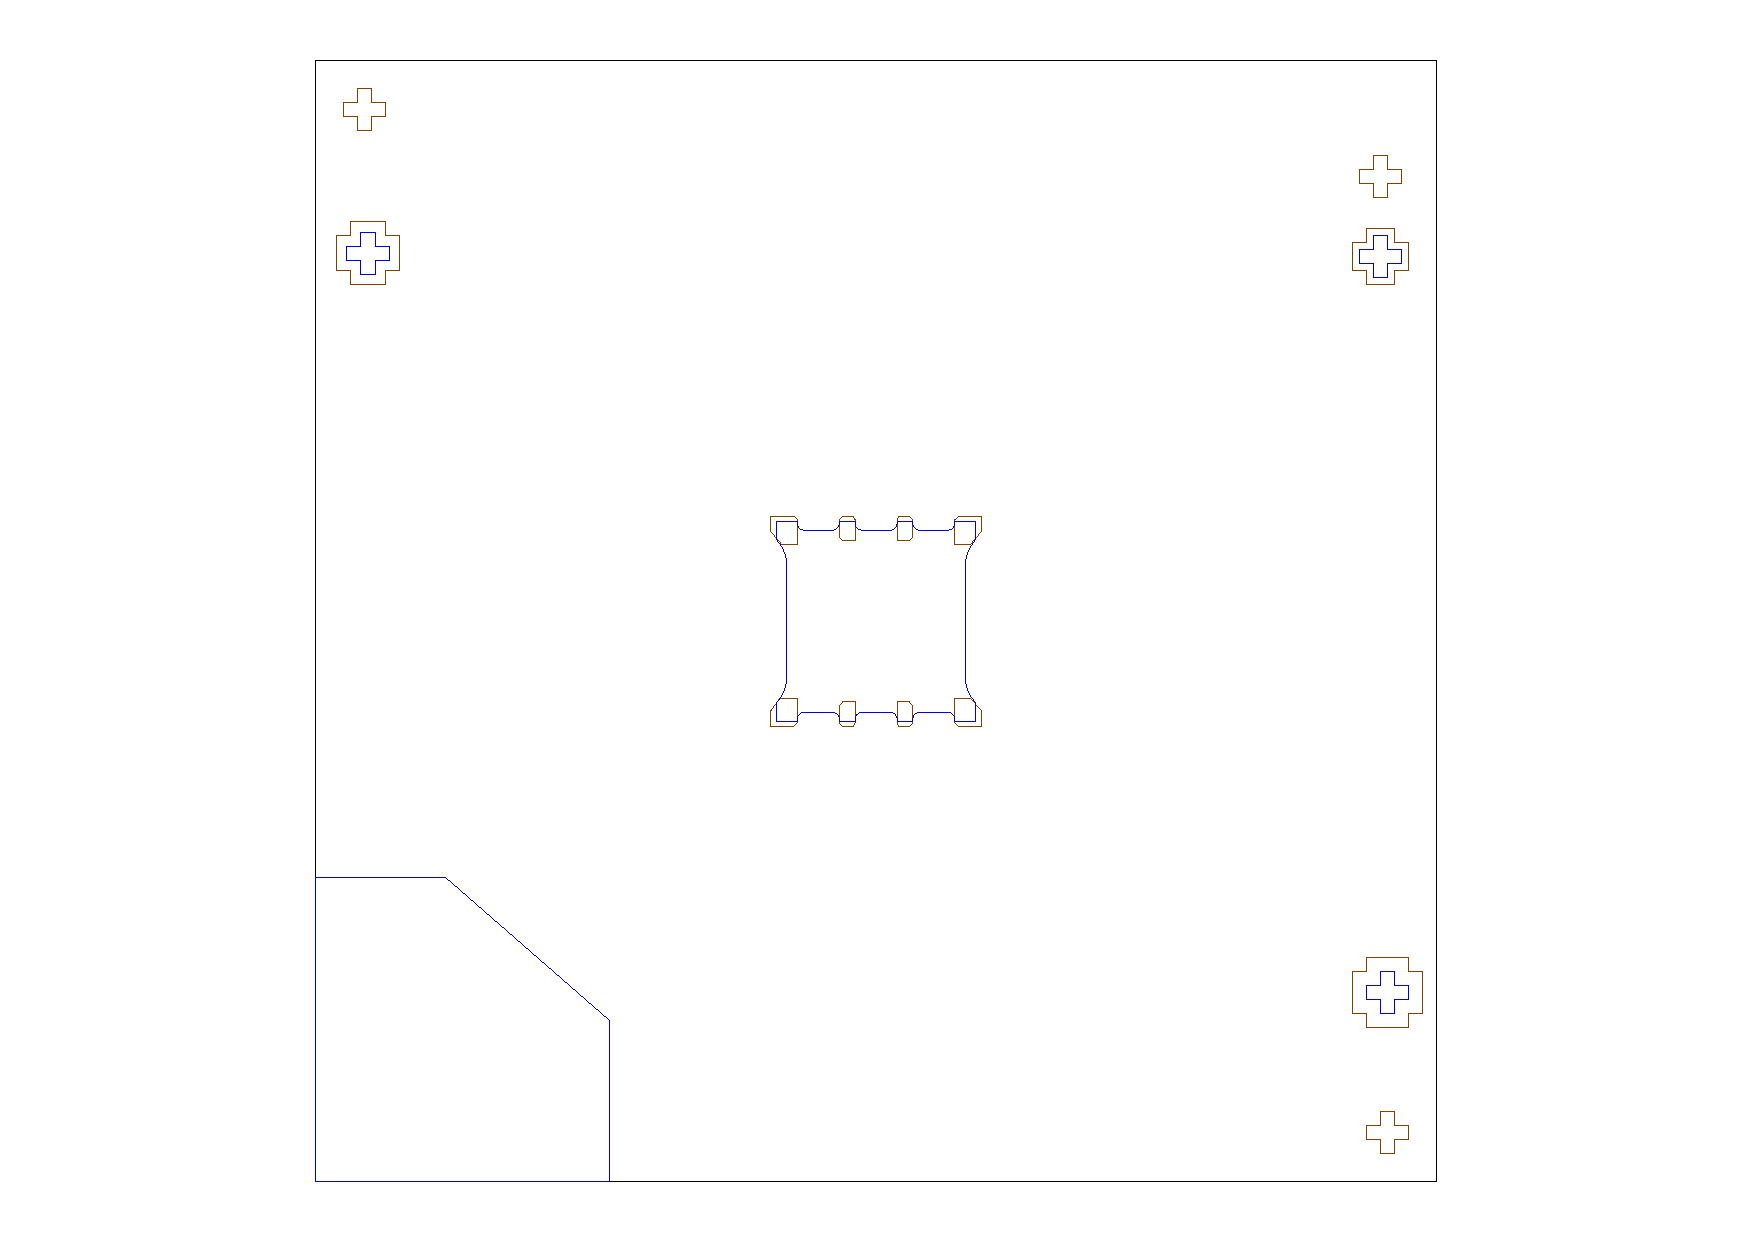
\includegraphics[scale=0.6]{fig/align1_1.pdf}
\caption{Picture of the geometry to expose. Can be used to write coordinates.} \label{align1}
\end{figure}

\newpage

\begin{figure} [h] \centering
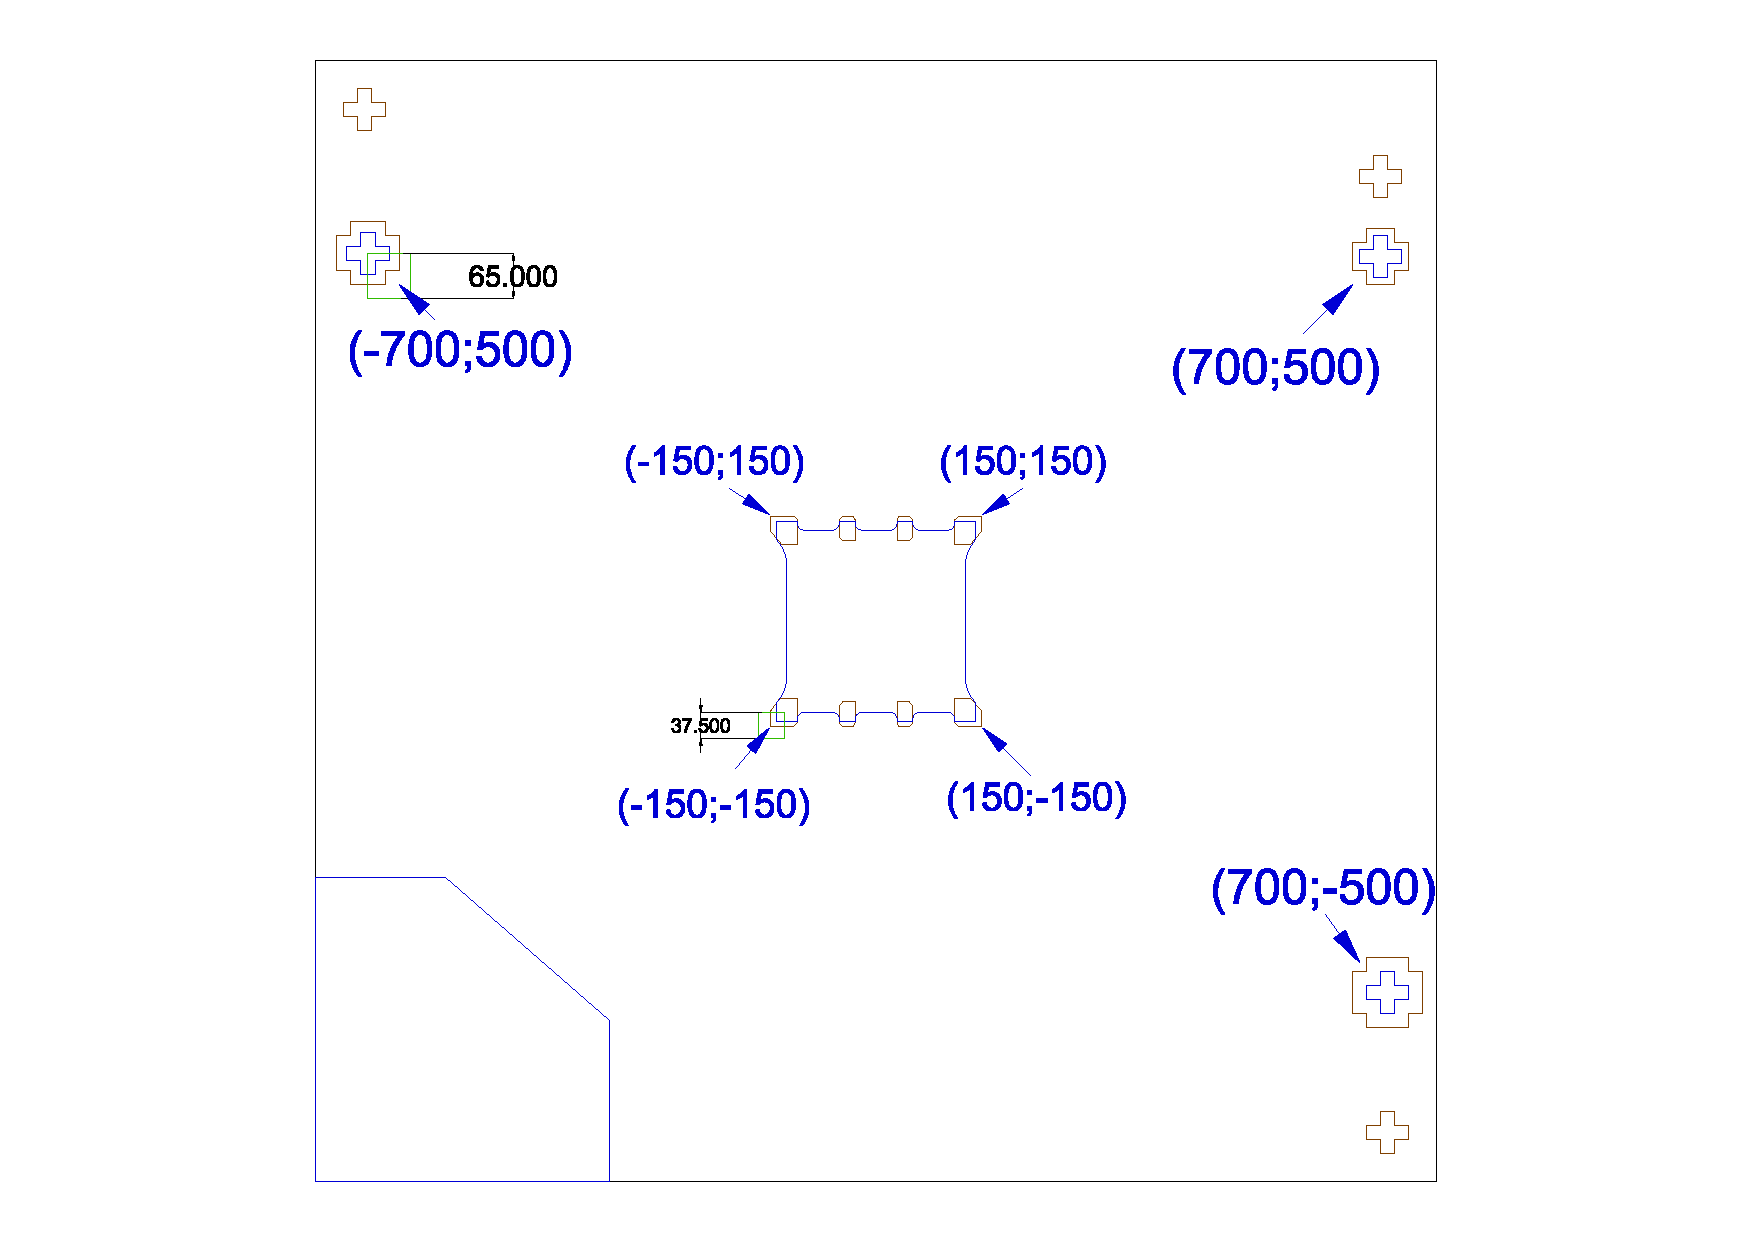
\includegraphics[scale=0.6]{fig/DD_Dots_V6_with_coord.pdf}
\caption{Marks coordinates for manual alignment. Coordinates won't change from one pattern to another, cause 
the marks are symmetric. Marks at the center are not to be used but in alignment problems (be careful about the exposing area).} \label{align1}
\end{figure}

\newpage

\begin{figure} [ht] \centering
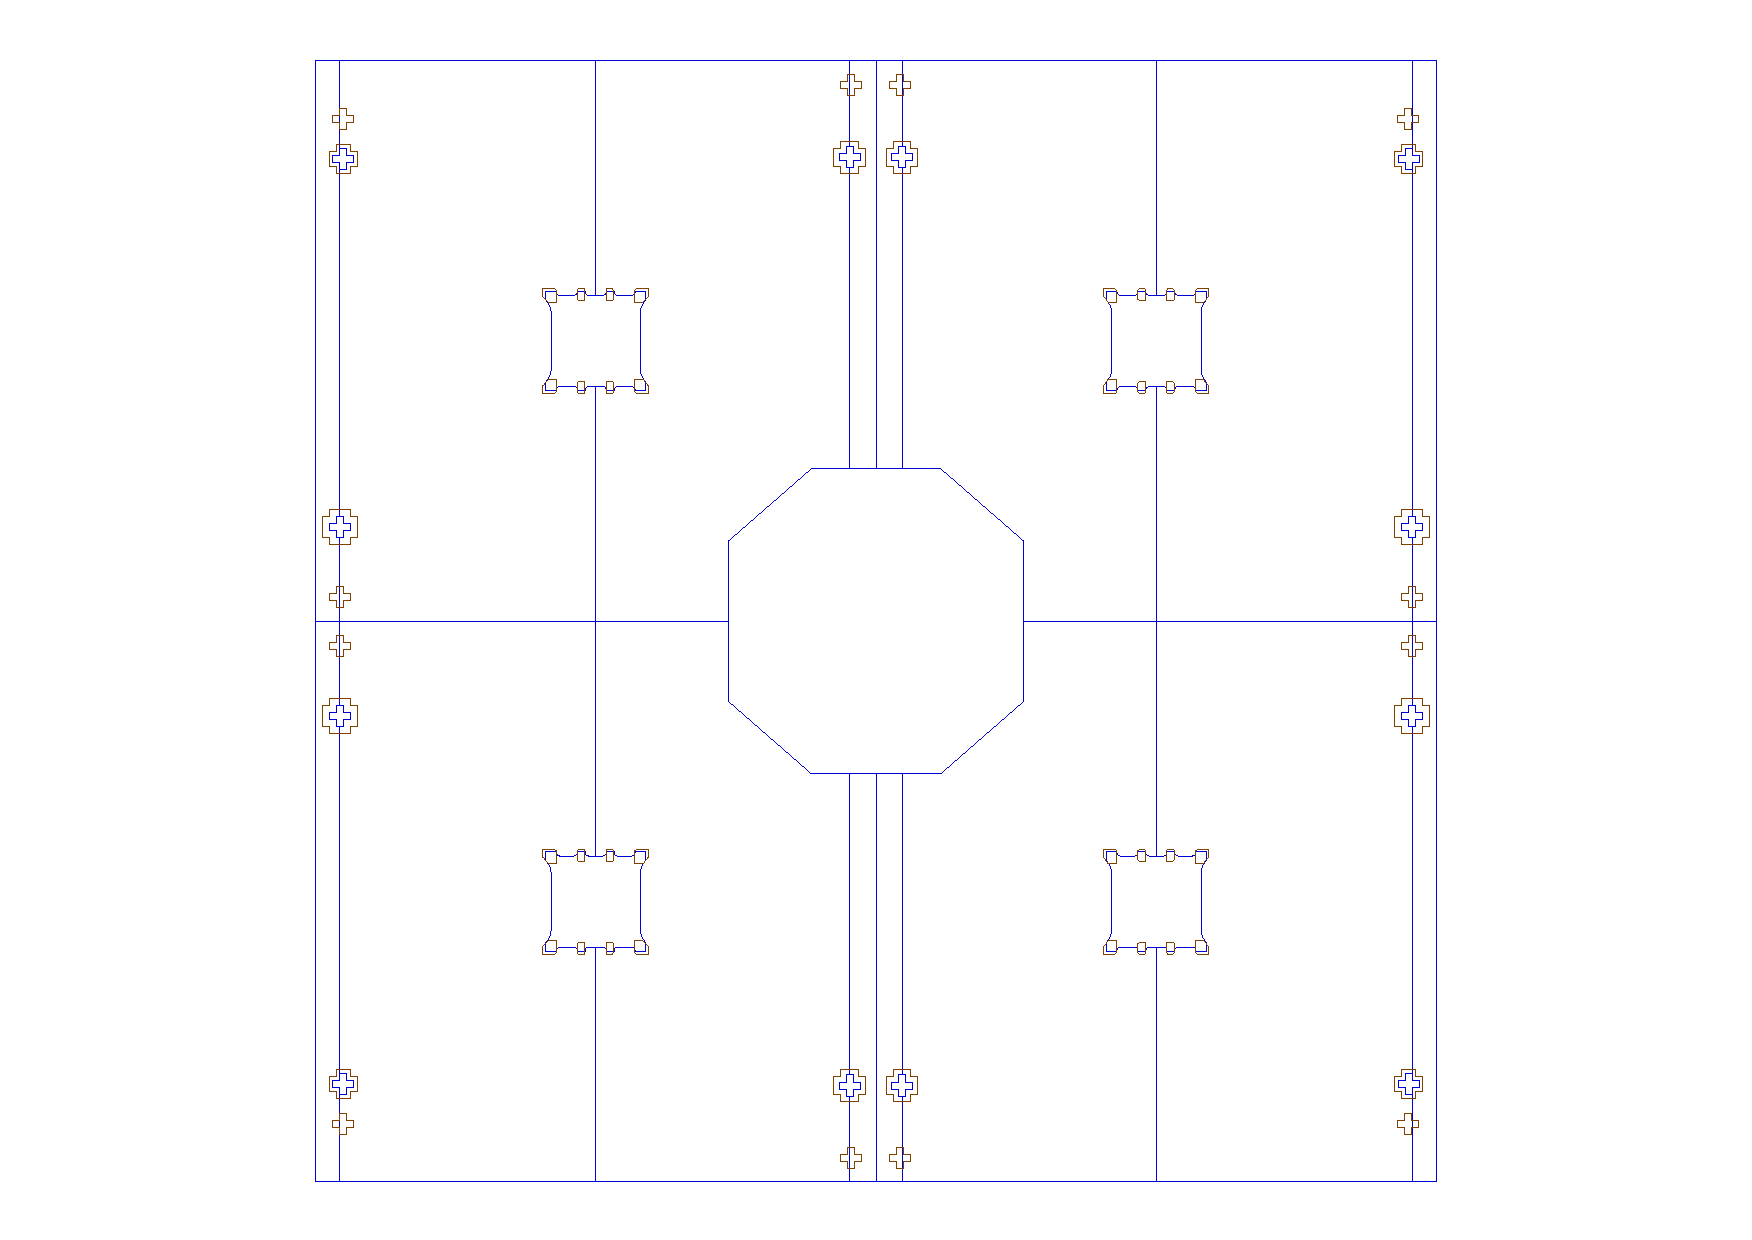
\includegraphics[scale=0.6]{fig/DD_Dots_V5_ebl_whole_mesa_ohmics.pdf}
\caption{Whole mask with mesa and ohmics} \label{align1}
\end{figure}

Size mesa : 840$\mu$m $\times$ 870$\mu$m. \\

UV coordinates of:\\

- Mark 1:~~~~~~~~~~~~~~~~~~~~~~~~~~~~~~~~~~~~~~~~~~~~~~~~ ; Mark 2: \\

- Mark 3:  \\

- center of mesa for gold balls: \\

- Ohmic corner 1:~~~~~~~~~~~~~~~~~~~~~~~~~~~~~~~~~~~~~~~~~; Ohmic corner 2:\\

- Ohmic corner 3:~~~~~~~~~~~~~~~~~~~~~~~~~~~~~~~~~~~~~~~~~; Ohmic corner 4:\\

\newpage

\section{Notes}

\newpage

\textbf{- Notes -}

\newpage

\textbf{- Notes -}

\end{document}
